\documentclass[border=4pt]{standalone}
\usepackage[T1]{fontenc}
\usepackage[scaled=0.92]{helvet}
\renewcommand{\familydefault}{\sfdefault}
\usepackage{tikz}\usetikzlibrary{arrows.meta,positioning,fit,backgrounds,calc,shapes.geometric}
\definecolor{navy}{HTML}{1F3A5F}\definecolor{ink}{HTML}{1E2633}\definecolor{muted}{HTML}{5B6573}
\definecolor{hair}{HTML}{C9D1DB}\definecolor{soft}{HTML}{E4EAF2}\definecolor{accent}{HTML}{C2410C}
\tikzset{
 box/.style={draw=navy, fill=soft, rounded corners=2pt, line width=0.7pt, align=center, font=\scriptsize, text=ink, inner sep=4pt},
 wbox/.style={draw=navy, fill=white, rounded corners=2pt, line width=0.7pt, align=center, font=\scriptsize, text=ink, inner sep=4pt},
 hbox/.style={draw=accent, fill=accent!8, rounded corners=2pt, line width=0.8pt, align=center, font=\scriptsize, text=ink, inner sep=4pt},
 title/.style={font=\scriptsize\bfseries, text=navy},
 dec/.style={diamond, aspect=2.2, draw=navy, fill=white, line width=0.7pt, align=center, font=\scriptsize, text=ink, inner sep=1pt},
 arr/.style={-{Stealth[length=5pt]}, draw=navy, line width=0.7pt},
 darr/.style={-{Stealth[length=5pt]}, draw=navy, line width=0.7pt, dashed},
 lab/.style={font=\tiny, text=muted, align=center},
}
\begin{document}

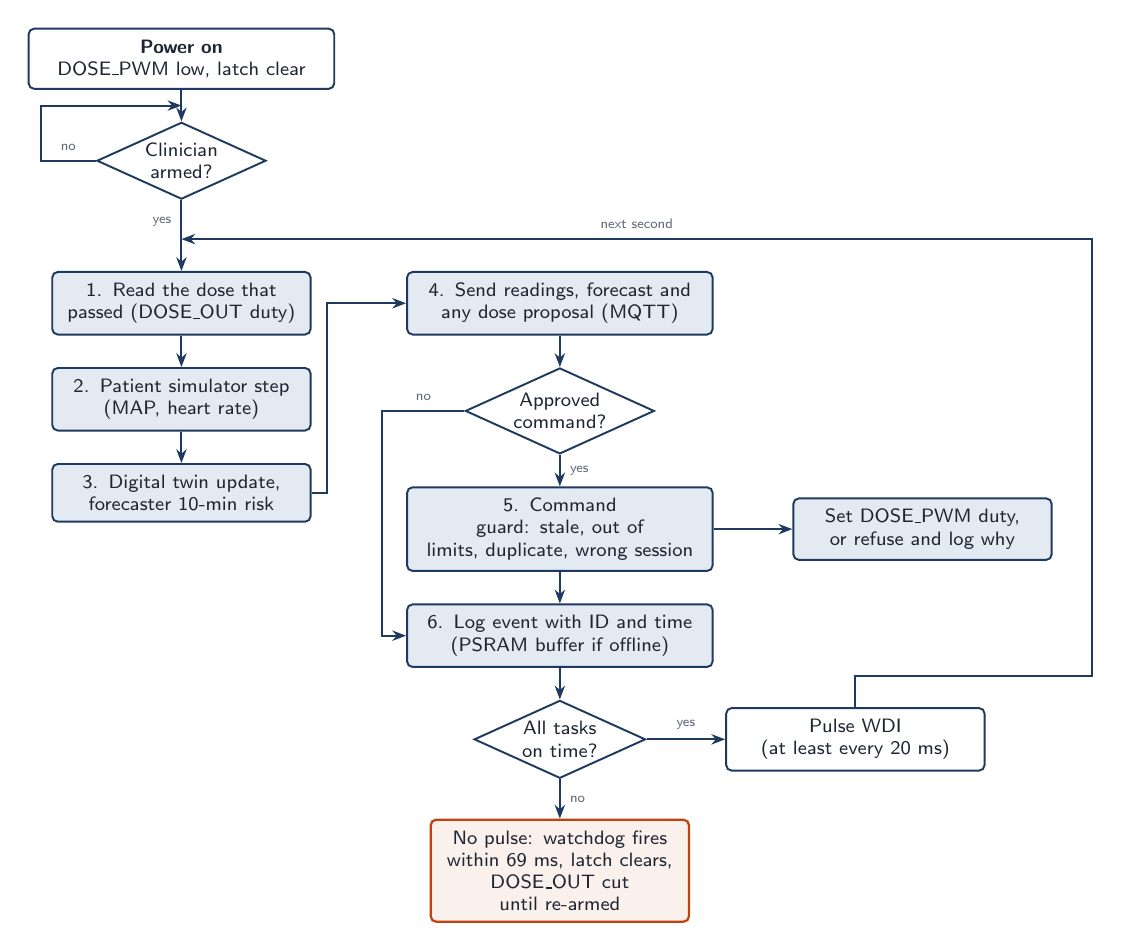
\begin{tikzpicture}[node distance=4mm]
\node[wbox, text width=36mm] (on) {\textbf{Power on}\\DOSE\_PWM low, latch clear};
\node[dec, below=4mm of on] (arm) {Clinician\\armed?};
\node[box, text width=30mm, below=9mm of arm] (rd) {1. Read the dose that\\passed (DOSE\_OUT duty)};
\node[box, text width=30mm, below=of rd] (sim) {2. Patient simulator step\\(MAP, heart rate)};
\node[box, text width=30mm, below=of sim] (tw) {3. Digital twin update,\\forecaster 10-min risk};
\node[box, text width=36mm, right=12mm of rd] (pr) {4. Send readings, forecast and\\any dose proposal (MQTT)};
\node[dec, below=4mm of pr] (cmd) {Approved\\command?};
\node[box, text width=36mm, below=4mm of cmd] (gd) {5. Command guard: stale, out of\\limits, duplicate, wrong session};
\node[box, text width=36mm, below=of gd] (lg) {6. Log event with ID and time\\(PSRAM buffer if offline)};
\node[dec, below=4mm of lg] (ok) {All tasks\\on time?};
\node[box, text width=30mm, right=10mm of gd] (set) {Set DOSE\_PWM duty,\\or refuse and log why};
\node[wbox, text width=30mm, right=10mm of ok] (kick) {Pulse WDI\\(at least every 20 ms)};
\node[hbox, text width=30mm, below=5mm of ok] (cut) {No pulse: watchdog fires\\within 69 ms, latch clears,\\DOSE\_OUT cut until re-armed};
\draw[arr] (on) -- coordinate[pos=0.5] (j1) (arm);
\draw[arr] (arm) -- coordinate[pos=0.55] (j2) node[lab, left, pos=0.3]{yes} (rd);
\draw[arr] (arm.west) -- node[lab, above]{no} ++(-7mm,0) |- (j1);
\draw[arr] (rd) -- (sim); \draw[arr] (sim) -- (tw);
\draw[arr] (tw.east) -- ++(2mm,0) |- (pr.west);
\draw[arr] (pr) -- (cmd);
\draw[arr] (cmd) -- node[lab, right]{yes} (gd);
\draw[arr] (cmd.west) -- node[lab, above]{no} ($(pr.west |- cmd.west)+(-3mm,0)$) |- (lg.west);
\draw[arr] (gd) -- (set);
\draw[arr] (gd) -- (lg); \draw[arr] (lg) -- (ok);
\draw[arr] (ok) -- node[lab, above]{yes} (kick);
\draw[arr] (ok) -- node[lab, right]{no} (cut);
\draw[arr] (kick.north) -- ++(0,4mm) -| ($(set.east)+(5mm,0)$) |- node[lab, above, pos=0.75]{next second} (j2);
\end{tikzpicture}
\end{document}
